\documentclass[tikz,border=5mm]{article}
\usepackage{tikz, pgfplots}
\usepackage[]{amsmath}
\usetikzlibrary{arrows}
\usepackage{pgfplots}
\pgfplotsset{width=8cm,compat=1.9}
\usetikzlibrary{pgfplots.dateplot}
\usepackage{pgfplotstable}
\usepackage{filecontents}
\usetikzlibrary{arrows}
\usetikzlibrary{plotmarks}
\usetikzlibrary{shapes.geometric}
\pgfplotsset{compat=1.12}
\begin{document}
\begin{figure}
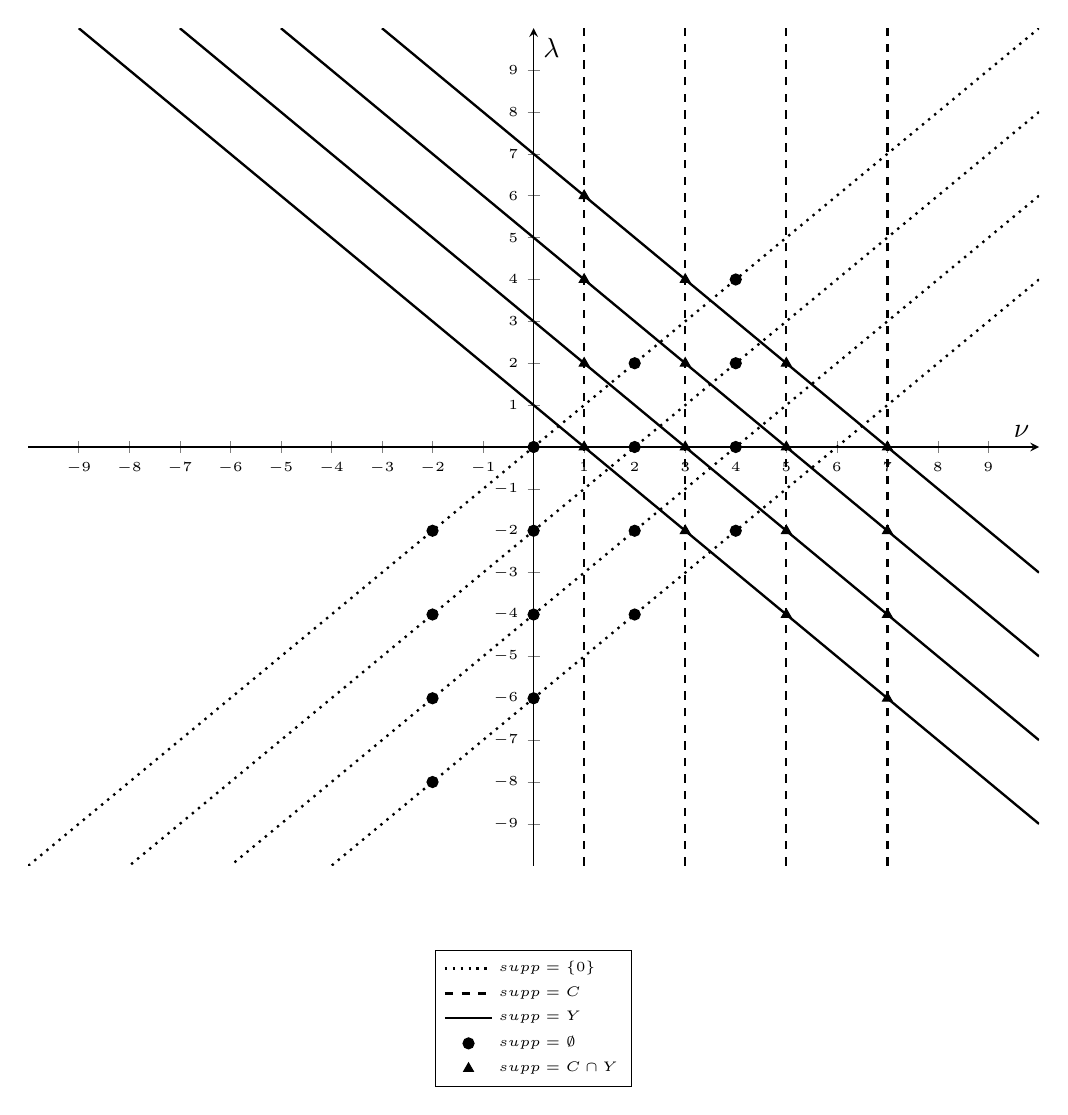
\begin{tikzpicture}
\begin{axis}[scale=2,
xlabel = $\nu$,ylabel = $\lambda$,
xmin=-10,xmax=10,ymin=-10,ymax=10,
label style={font=\tiny},tick label style={font=\tiny},
label style ={at={(ticklabel cs:1.5)}},
xtick={-9,-8,...,9},
ytick={-9,-8,...,9},
legend style={at={(0.5,-0.1)},anchor=north,font=\tiny},
axis lines=middle,legend cell align=left]
(-1 1 -6)
\draw[line width=0.3mm,style=dotted] (10.0,4.0) -- (-4.0,-10.0);
(-1 1 -4)
\draw[line width=0.3mm,style=dotted] (10.0,6.0) -- (-6.0,-10.0);
(-1 1 -2)
\draw[line width=0.3mm,style=dotted] (10.0,8.0) -- (-8.0,-10.0);
(-1 1 0)
\draw[line width=0.3mm,style=dotted] (-10.0,-10.0) -- (10.0,10.0);
(1 0 7)
\draw[line width=0.3mm,style=dashed] (7.0,-10.0) -- (7.0,10.0);
(1 0 5)
\draw[line width=0.3mm,style=dashed] (5.0,-10.0) -- (5.0,10.0);
(1 0 3)
\draw[line width=0.3mm,style=dashed] (3.0,-10.0) -- (3.0,10.0);
(1 0 1)
\draw[line width=0.3mm,style=dashed] (1.0,-10.0) -- (1.0,10.0);
(1 1 1)
\draw[line width=0.3mm] (10.0,-9.0) -- (-9.0,10.0);
(1 1 3)
\draw[line width=0.3mm] (10.0,-7.0) -- (-7.0,10.0);
(1 1 5)
\draw[line width=0.3mm] (10.0,-5.0) -- (-5.0,10.0);
(1 1 7)
\draw[line width=0.3mm] (10.0,-3.0) -- (-3.0,10.0);
\node at (-2.0,-2.0) {\pgfuseplotmark{*}};
\node at (0.0,0.0) {\pgfuseplotmark{*}};
\node at (4.0,4.0) {\pgfuseplotmark{*}};
\node at (2.0,2.0) {\pgfuseplotmark{*}};
\node at (-2.0,-4.0) {\pgfuseplotmark{*}};
\node at (0.0,-2.0) {\pgfuseplotmark{*}};
\node at (4.0,2.0) {\pgfuseplotmark{*}};
\node at (2.0,0.0) {\pgfuseplotmark{*}};
\node at (-2.0,-6.0) {\pgfuseplotmark{*}};
\node at (0.0,-4.0) {\pgfuseplotmark{*}};
\node at (4.0,0.0) {\pgfuseplotmark{*}};
\node at (2.0,-2.0) {\pgfuseplotmark{*}};
\node at (-2.0,-8.0) {\pgfuseplotmark{*}};
\node at (0.0,-6.0) {\pgfuseplotmark{*}};
\node at (4.0,-2.0) {\pgfuseplotmark{*}};
\node at (2.0,-4.0) {\pgfuseplotmark{*}};
\node at (7.0,0.0) {\pgfuseplotmark{triangle*}};
\node at (5.0,2.0) {\pgfuseplotmark{triangle*}};
\node at (3.0,4.0) {\pgfuseplotmark{triangle*}};
\node at (1.0,6.0) {\pgfuseplotmark{triangle*}};
\node at (7.0,-2.0) {\pgfuseplotmark{triangle*}};
\node at (5.0,0.0) {\pgfuseplotmark{triangle*}};
\node at (3.0,2.0) {\pgfuseplotmark{triangle*}};
\node at (1.0,4.0) {\pgfuseplotmark{triangle*}};
\node at (7.0,-4.0) {\pgfuseplotmark{triangle*}};
\node at (5.0,-2.0) {\pgfuseplotmark{triangle*}};
\node at (3.0,0.0) {\pgfuseplotmark{triangle*}};
\node at (1.0,2.0) {\pgfuseplotmark{triangle*}};
\node at (7.0,-6.0) {\pgfuseplotmark{triangle*}};
\node at (5.0,-4.0) {\pgfuseplotmark{triangle*}};
\node at (3.0,-2.0) {\pgfuseplotmark{triangle*}};
\node at (1.0,0.0) {\pgfuseplotmark{triangle*}};
\addlegendimage{line width=0.3mm,style=dotted}
\addlegendentry{$supp=\{0\}$}
\addlegendimage{line width=0.3mm,style=dashed}
\addlegendentry{$supp=C$}
\addlegendimage{line width=0.3mm}
\addlegendentry{$supp=Y$}
\addlegendimage{only marks, mark=*}
\addlegendentry{$supp=\emptyset$}
\addlegendimage{only marks, mark=triangle*}
\addlegendentry{$supp=C\cap Y$}
\end{axis}
\end{tikzpicture}

\caption{support of regular SBO for $(p,q)=(3,5)$}
\end{figure}
\end{document}
%having two families of lines
%moving bounds and axes appropriately
%legend
